% Options for packages loaded elsewhere
\PassOptionsToPackage{unicode}{hyperref}
\PassOptionsToPackage{hyphens}{url}
%
\documentclass[
]{article}
\usepackage{amsmath,amssymb}
\usepackage{lmodern}
\usepackage{ifxetex,ifluatex}
\ifnum 0\ifxetex 1\fi\ifluatex 1\fi=0 % if pdftex
  \usepackage[T1]{fontenc}
  \usepackage[utf8]{inputenc}
  \usepackage{textcomp} % provide euro and other symbols
\else % if luatex or xetex
  \usepackage{unicode-math}
  \defaultfontfeatures{Scale=MatchLowercase}
  \defaultfontfeatures[\rmfamily]{Ligatures=TeX,Scale=1}
\fi
% Use upquote if available, for straight quotes in verbatim environments
\IfFileExists{upquote.sty}{\usepackage{upquote}}{}
\IfFileExists{microtype.sty}{% use microtype if available
  \usepackage[]{microtype}
  \UseMicrotypeSet[protrusion]{basicmath} % disable protrusion for tt fonts
}{}
\makeatletter
\@ifundefined{KOMAClassName}{% if non-KOMA class
  \IfFileExists{parskip.sty}{%
    \usepackage{parskip}
  }{% else
    \setlength{\parindent}{0pt}
    \setlength{\parskip}{6pt plus 2pt minus 1pt}}
}{% if KOMA class
  \KOMAoptions{parskip=half}}
\makeatother
\usepackage{xcolor}
\IfFileExists{xurl.sty}{\usepackage{xurl}}{} % add URL line breaks if available
\IfFileExists{bookmark.sty}{\usepackage{bookmark}}{\usepackage{hyperref}}
\hypersetup{
  pdftitle={Species ID Guide Template},
  pdfauthor={Carys Hughes},
  hidelinks,
  pdfcreator={LaTeX via pandoc}}
\urlstyle{same} % disable monospaced font for URLs
\usepackage[margin=1in]{geometry}
\usepackage{color}
\usepackage{fancyvrb}
\newcommand{\VerbBar}{|}
\newcommand{\VERB}{\Verb[commandchars=\\\{\}]}
\DefineVerbatimEnvironment{Highlighting}{Verbatim}{commandchars=\\\{\}}
% Add ',fontsize=\small' for more characters per line
\usepackage{framed}
\definecolor{shadecolor}{RGB}{248,248,248}
\newenvironment{Shaded}{\begin{snugshade}}{\end{snugshade}}
\newcommand{\AlertTok}[1]{\textcolor[rgb]{0.94,0.16,0.16}{#1}}
\newcommand{\AnnotationTok}[1]{\textcolor[rgb]{0.56,0.35,0.01}{\textbf{\textit{#1}}}}
\newcommand{\AttributeTok}[1]{\textcolor[rgb]{0.77,0.63,0.00}{#1}}
\newcommand{\BaseNTok}[1]{\textcolor[rgb]{0.00,0.00,0.81}{#1}}
\newcommand{\BuiltInTok}[1]{#1}
\newcommand{\CharTok}[1]{\textcolor[rgb]{0.31,0.60,0.02}{#1}}
\newcommand{\CommentTok}[1]{\textcolor[rgb]{0.56,0.35,0.01}{\textit{#1}}}
\newcommand{\CommentVarTok}[1]{\textcolor[rgb]{0.56,0.35,0.01}{\textbf{\textit{#1}}}}
\newcommand{\ConstantTok}[1]{\textcolor[rgb]{0.00,0.00,0.00}{#1}}
\newcommand{\ControlFlowTok}[1]{\textcolor[rgb]{0.13,0.29,0.53}{\textbf{#1}}}
\newcommand{\DataTypeTok}[1]{\textcolor[rgb]{0.13,0.29,0.53}{#1}}
\newcommand{\DecValTok}[1]{\textcolor[rgb]{0.00,0.00,0.81}{#1}}
\newcommand{\DocumentationTok}[1]{\textcolor[rgb]{0.56,0.35,0.01}{\textbf{\textit{#1}}}}
\newcommand{\ErrorTok}[1]{\textcolor[rgb]{0.64,0.00,0.00}{\textbf{#1}}}
\newcommand{\ExtensionTok}[1]{#1}
\newcommand{\FloatTok}[1]{\textcolor[rgb]{0.00,0.00,0.81}{#1}}
\newcommand{\FunctionTok}[1]{\textcolor[rgb]{0.00,0.00,0.00}{#1}}
\newcommand{\ImportTok}[1]{#1}
\newcommand{\InformationTok}[1]{\textcolor[rgb]{0.56,0.35,0.01}{\textbf{\textit{#1}}}}
\newcommand{\KeywordTok}[1]{\textcolor[rgb]{0.13,0.29,0.53}{\textbf{#1}}}
\newcommand{\NormalTok}[1]{#1}
\newcommand{\OperatorTok}[1]{\textcolor[rgb]{0.81,0.36,0.00}{\textbf{#1}}}
\newcommand{\OtherTok}[1]{\textcolor[rgb]{0.56,0.35,0.01}{#1}}
\newcommand{\PreprocessorTok}[1]{\textcolor[rgb]{0.56,0.35,0.01}{\textit{#1}}}
\newcommand{\RegionMarkerTok}[1]{#1}
\newcommand{\SpecialCharTok}[1]{\textcolor[rgb]{0.00,0.00,0.00}{#1}}
\newcommand{\SpecialStringTok}[1]{\textcolor[rgb]{0.31,0.60,0.02}{#1}}
\newcommand{\StringTok}[1]{\textcolor[rgb]{0.31,0.60,0.02}{#1}}
\newcommand{\VariableTok}[1]{\textcolor[rgb]{0.00,0.00,0.00}{#1}}
\newcommand{\VerbatimStringTok}[1]{\textcolor[rgb]{0.31,0.60,0.02}{#1}}
\newcommand{\WarningTok}[1]{\textcolor[rgb]{0.56,0.35,0.01}{\textbf{\textit{#1}}}}
\usepackage{graphicx}
\makeatletter
\def\maxwidth{\ifdim\Gin@nat@width>\linewidth\linewidth\else\Gin@nat@width\fi}
\def\maxheight{\ifdim\Gin@nat@height>\textheight\textheight\else\Gin@nat@height\fi}
\makeatother
% Scale images if necessary, so that they will not overflow the page
% margins by default, and it is still possible to overwrite the defaults
% using explicit options in \includegraphics[width, height, ...]{}
\setkeys{Gin}{width=\maxwidth,height=\maxheight,keepaspectratio}
% Set default figure placement to htbp
\makeatletter
\def\fps@figure{htbp}
\makeatother
\setlength{\emergencystretch}{3em} % prevent overfull lines
\providecommand{\tightlist}{%
  \setlength{\itemsep}{0pt}\setlength{\parskip}{0pt}}
\setcounter{secnumdepth}{-\maxdimen} % remove section numbering
\usepackage[font=small,format=plain,labelfont=bf,up,textfont=normal,up,justification=justified,singlelinecheck=false]{caption}
\usepackage{booktabs}
\usepackage{longtable}
\usepackage{array}
\usepackage{multirow}
\usepackage{wrapfig}
\usepackage{float}
\usepackage{colortbl}
\usepackage{pdflscape}
\usepackage{tabu}
\usepackage{threeparttable}
\usepackage{threeparttablex}
\usepackage[normalem]{ulem}
\usepackage{makecell}
\usepackage{xcolor}
\ifluatex
  \usepackage{selnolig}  % disable illegal ligatures
\fi

\title{Species ID Guide Template}
\author{Carys Hughes}
\date{10/17/2021}

\begin{document}
\maketitle

\begin{Shaded}
\begin{Highlighting}[]
\FunctionTok{library}\NormalTok{(kableExtra)}
\FunctionTok{library}\NormalTok{(knitr)}
\FunctionTok{library}\NormalTok{(tidyverse)}
\end{Highlighting}
\end{Shaded}

\begin{verbatim}
## -- Attaching packages --------------------------------------- tidyverse 1.3.1 --
\end{verbatim}

\begin{verbatim}
## v ggplot2 3.3.5     v purrr   0.3.4
## v tibble  3.1.4     v dplyr   1.0.7
## v tidyr   1.1.3     v stringr 1.4.0
## v readr   2.0.1     v forcats 0.5.1
\end{verbatim}

\begin{verbatim}
## -- Conflicts ------------------------------------------ tidyverse_conflicts() --
## x dplyr::filter()     masks stats::filter()
## x dplyr::group_rows() masks kableExtra::group_rows()
## x dplyr::lag()        masks stats::lag()
\end{verbatim}

\begin{Shaded}
\begin{Highlighting}[]
\FunctionTok{library}\NormalTok{(here)}
\end{Highlighting}
\end{Shaded}

\begin{verbatim}
## here() starts at /Users/caryshughes/GitHub/species-id-guide-CarysH11
\end{verbatim}

\begin{Shaded}
\begin{Highlighting}[]
\FunctionTok{library}\NormalTok{(tinytex)}

\NormalTok{barnacle\_info\_table }\OtherTok{=} \FunctionTok{read\_csv}\NormalTok{(}\FunctionTok{here}\NormalTok{(}\StringTok{"./data/barnacle\_info\_table.csv"}\NormalTok{))}
\end{Highlighting}
\end{Shaded}

\begin{verbatim}
## Rows: 4 Columns: 6
\end{verbatim}

\begin{verbatim}
## -- Column specification --------------------------------------------------------
## Delimiter: ","
## chr (6): Scientific_name, Common_name, Size, Morphology, Trophic_role, Repro...
\end{verbatim}

\begin{verbatim}
## 
## i Use `spec()` to retrieve the full column specification for this data.
## i Specify the column types or set `show_col_types = FALSE` to quiet this message.
\end{verbatim}

\begin{Shaded}
\begin{Highlighting}[]
\NormalTok{barnacle\_info\_table }\OtherTok{=} \FunctionTok{data.frame}\NormalTok{(barnacle\_info\_table)}

\CommentTok{\# write custom function to display the table how we want}
\NormalTok{ knit\_table }\OtherTok{=} \ControlFlowTok{function}\NormalTok{(df)\{}
\NormalTok{     df }\OtherTok{=} \FunctionTok{data.frame}\NormalTok{(}\FunctionTok{lapply}\NormalTok{(df, }\ControlFlowTok{function}\NormalTok{(x) \{}\FunctionTok{gsub}\NormalTok{(}\StringTok{"\textless{}br\textgreater{}"}\NormalTok{, }\StringTok{"}\SpecialCharTok{\textbackslash{}n}\StringTok{"}\NormalTok{, x)\}), }\AttributeTok{stringsAsFactors =}\NormalTok{ F)}
 
\NormalTok{       df }\SpecialCharTok{\%\textgreater{}\%} 
\NormalTok{     dplyr}\SpecialCharTok{::}\FunctionTok{mutate\_all}\NormalTok{(linebreak) }\SpecialCharTok{\%\textgreater{}\%} 
\NormalTok{     kableExtra}\SpecialCharTok{::}\FunctionTok{kable}\NormalTok{(}\StringTok{"latex"}\NormalTok{, }
           \AttributeTok{booktabs =} \ConstantTok{TRUE}\NormalTok{, }
           \AttributeTok{escape =} \ConstantTok{FALSE}\NormalTok{, }
           \AttributeTok{longtable =} \ConstantTok{FALSE}\NormalTok{) }\SpecialCharTok{\%\textgreater{}\%} 
\NormalTok{     kableExtra}\SpecialCharTok{::}\FunctionTok{kable\_styling}\NormalTok{(}\AttributeTok{latex\_options =} \StringTok{"scale\_down"}\NormalTok{, }
                   \AttributeTok{full\_width =} \ConstantTok{FALSE}\NormalTok{)  }\SpecialCharTok{\%\textgreater{}\%} 
     \FunctionTok{column\_spec}\NormalTok{(}\DecValTok{1}\NormalTok{, }\AttributeTok{width =} \StringTok{"5em"}\NormalTok{) }\SpecialCharTok{\%\textgreater{}\%} 
     \FunctionTok{column\_spec}\NormalTok{(}\DecValTok{2}\NormalTok{, }\AttributeTok{width =} \StringTok{"5em"}\NormalTok{)}
\NormalTok{ \}}
 \FunctionTok{knit\_table}\NormalTok{(barnacle\_info\_table)}
\end{Highlighting}
\end{Shaded}

\begin{table}
\centering
\resizebox{\linewidth}{!}{
\begin{tabular}{>{\raggedright\arraybackslash}p{5em}>{\raggedright\arraybackslash}p{5em}llll}
\toprule
Scientific_name & Common_name & Size & Morphology & Trophic_role & Reproductive_mode\\
\midrule
Semibalanus cariosus & Thatched barnacle & \makecell[l]{Height: 18.8 mm\\\\Diameter: 16.6 mm} & \makecell[l]{Thatched lines on barnacle\\\\White, grey, brown, greenish in colour\\\\Grow tall in crowded areas and volcano shaped in uncrowded areas} & \makecell[l]{Suspension feeders: collect plankton and detritus using cirri\\\\Predators are sea stars, whelks, snails and birds} & \makecell[l]{Hermaphroditic\\\\Pheromones stimulate larval hatching\\\\Brood eggs in the winter and larvae settle in the spring}\\
Chthamalus dalli & Small acorn barnacle & \makecell[c]{Height: 1mm\\\\Diameter: 3.5 mm} & \makecell[c]{Brown-grey in colour\\\\Smooth surface} & \makecell[c]{Suspension feeders: collect plankton and detritus using cirri\\\\Predators are snails and sea stars} & \makecell[c]{Hermaphroditic\\\\Reproduce several times per year\\\\Brood size of 12000 eggs\\\\Broods can remain within barnacle up to 6 months\\\\The Isopod Cryptothis balani may inhibit reproduction}\\
Pollicipes polymerus & Gooseneck barnacle & \makecell[r]{Height: 8 mm\\\\Diameter: 11.4 mm} & \makecell[r]{White protective plates (5 large, many small)\\\\Fleshy peduncle} & \makecell[r]{Suspension feeders: collect plankton and detritus using cirri\\\\Predators are sea stars and birds} & \makecell[r]{Hermaphroditic\\\\Cross-fertilize through pseudocopulation and sperm acquisition from the water\\\\Reproduce from April to October in the PNW\\\\Can produce 4 broods each year\\\\20000 embryos per brood}\\
Balanus glandula & Acorn barnacle & \makecell[l]{Height: 3.9 mm\\\\Diameter: 7 mm} & \makecell[l]{Volcano shaped when isolated\\\\Tall and thin when crowded\\\\Black lining inside plates\\\\White or greyish white\\\\Longitudinal ribbing sometimes visible} & \makecell[l]{Suspension feeders: collect plankton and detritus using cirri\\\\Predators are snails and barnacle nudibranchs} & \makecell[l]{Hermaphroditic\\\\Live up to 7 years}\\
\bottomrule
\end{tabular}}
\end{table}

\newpage

\hypertarget{eubalaena-australis-southern-right-whale}{%
\section{\texorpdfstring{\emph{Eubalaena australis} (Southern right
whale)}{Eubalaena australis (Southern right whale)}}\label{eubalaena-australis-southern-right-whale}}

\hypertarget{description}{%
\subsection{Description}\label{description}}

These stocky whales have extremely large heads, which can be over
one-fourth of the body length. The mouthline is bowed and the rostrum is
arched. Text text text text. \textbf{Bold text bold text bold text.}
\emph{Italicized text italicized text italicized text}. Text text text
text. \textbf{Bold text bold text bold text.} \emph{Italicized text
italicized text italicized text}. Text text text text. \textbf{Bold text
bold text bold text.} \emph{Italicized text italicized text italicized
text}. Text text text text. \textbf{Bold text bold text bold text.}
\emph{Italicized text italicized text italicized text}. Text text text
text. \textbf{Bold text bold text bold text.} \emph{Italicized text
italicized text italicized text}. Text text text text. \textbf{Bold text
bold text bold text.} \emph{Italicized text italicized text italicized
text}. Text text text text. \textbf{Bold text bold text bold text.}
\emph{Italicized text italicized text italicized text}. Text text text
text. \textbf{Bold text bold text bold text.} \emph{Italicized text
italicized text italicized text}. Text text text text. \textbf{Bold text
bold text bold text.} \emph{Italicized text italicized text italicized
text}. Text text text text. \textbf{Bold text bold text bold text.}
\emph{Italicized text italicized text italicized text}. Text text text
text. \textbf{Bold text bold text bold text.} \emph{Italicized text
italicized text italicized text}.

\newpage

\hypertarget{figures}{%
\subsection{Figures}\label{figures}}

\begin{figure}

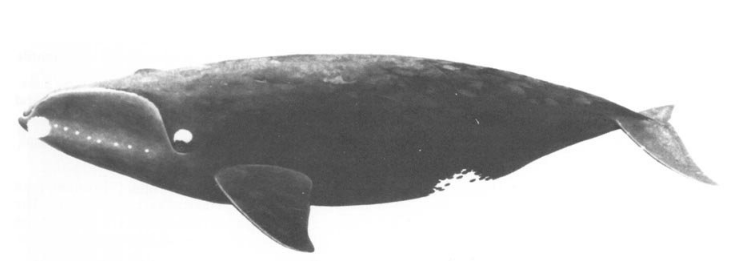
\includegraphics[width=0.5\linewidth,height=0.3\textheight]{/Users/caryshughes/GitHub/species-id-guide-CarysH11/images/southern-right} \hfill{}

\caption{This is the southern right whale, figure is centered.}\label{fig:southern-right-whale}
\end{figure}

\begin{figure}

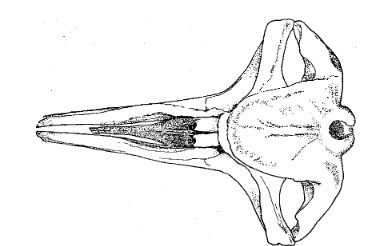
\includegraphics[width=0.5\linewidth,height=0.3\textheight]{/Users/caryshughes/GitHub/species-id-guide-CarysH11/images/southern-right-skull} \hfill{}

\caption{This is the skull of the southern right whale skull (dorsal view), figure is left-aligned.}\label{fig:southern-right-whale-skull}
\end{figure}

\begin{figure}

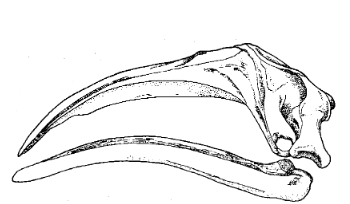
\includegraphics[width=0.5\linewidth,height=0.3\textheight]{/Users/caryshughes/GitHub/species-id-guide-CarysH11/images/southern-right-skull-lateral} \hfill{}

\caption{This is the skull of the southern right whale skull (lateral view), figure is left-aligned.}\label{fig:southern-right-whale-skull-lateral}
\end{figure}

\newpage

\hypertarget{questions}{%
\subsection{Questions}\label{questions}}

\begin{enumerate}
\def\labelenumi{\arabic{enumi}.}
\tightlist
\item
  Very interesting and useful question
\item
  Another wildly helpful question
\item
  A third, MOST fascinating question
\end{enumerate}

\hypertarget{balaena-mysticetus-bowhead-whale}{%
\section{\texorpdfstring{\emph{Balaena mysticetus} (Bowhead
whale)}{Balaena mysticetus (Bowhead whale)}}\label{balaena-mysticetus-bowhead-whale}}

\hypertarget{description-1}{%
\subsection{Description}\label{description-1}}

Bowhead whales are very rotund, but often have a distinct ``neck''
region. The head is large\ldots{} Text text text text. \textbf{Bold text
bold text bold text.} \emph{Italicized text italicized text italicized
text}. Text text text text. \textbf{Bold text bold text bold text.}
\emph{Italicized text italicized text italicized text}. Text text text
text. \textbf{Bold text bold text bold text.} \emph{Italicized text
italicized text italicized text}. Text text text text. \textbf{Bold text
bold text bold text.} \emph{Italicized text italicized text italicized
text}. Text text text text. \textbf{Bold text bold text bold text.}
\emph{Italicized text italicized text italicized text}. Text text text
text. \textbf{Bold text bold text bold text.} \emph{Italicized text
italicized text italicized text}. Text text text text. \textbf{Bold text
bold text bold text.} \emph{Italicized text italicized text italicized
text}. Text text text text. \textbf{Bold text bold text bold text.}
\emph{Italicized text italicized text italicized text}. Text text text
text. \textbf{Bold text bold text bold text.} \emph{Italicized text
italicized text italicized text}. Text text text text. \textbf{Bold text
bold text bold text.} \emph{Italicized text italicized text italicized
text}. Text text text text. \textbf{Bold text bold text bold text.}
\emph{Italicized text italicized text italicized text}. Text text text
text. \textbf{Bold text bold text bold text.} \emph{Italicized text
italicized text italicized text}.

\newpage

\hypertarget{figures-1}{%
\subsection{Figures}\label{figures-1}}

\begin{figure}
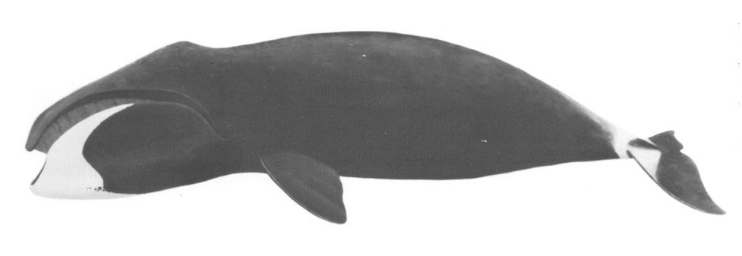
\includegraphics[width=0.5\linewidth,height=0.3\textheight]{/Users/caryshughes/GitHub/species-id-guide-CarysH11/images/bowhead} \caption{This is the bowhead whale, figure is centered.}\label{fig:bowhead-whale}
\end{figure}

\begin{figure}
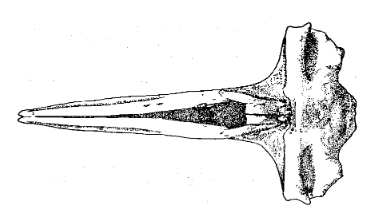
\includegraphics[width=0.5\linewidth,height=0.3\textheight]{/Users/caryshughes/GitHub/species-id-guide-CarysH11/images/bowhead-skull} \caption{This is the skull of the bowhead whale skull, figure is centered.}\label{fig:bowhead-whale-skull}
\end{figure}

\begin{figure}
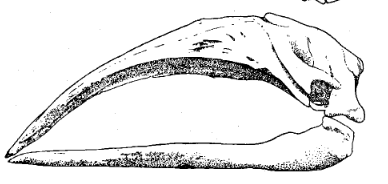
\includegraphics[width=0.5\linewidth,height=0.3\textheight]{/Users/caryshughes/GitHub/species-id-guide-CarysH11/images/bowhead-skull-lateral} \caption{This is the skull of the bowhead whale skull, figure is centered.}\label{fig:bowhead-whale-skull-lateral}
\end{figure}

\newpage

\hypertarget{questions-1}{%
\subsection{Questions}\label{questions-1}}

\begin{enumerate}
\def\labelenumi{\arabic{enumi}.}
\tightlist
\item
  Very interesting and useful question
\item
  Another wildly helpful question
\item
  A third, MOST fascinating question
\end{enumerate}

\newpage

\hypertarget{supplemental-information}{%
\section{Supplemental Information}\label{supplemental-information}}

\begin{table}

\caption{\label{tab:unnamed-chunk-2}Whale morphometrics and other infomration.}
\centering
\begin{tabular}[t]{l|l|l|l|l|l}
\hline
Species & Length & Weight & Trophic Role & Diet & Reproduction\\
\hline
Bowhead whale & 18..7-20.8 & 81542.79 - 90700 & predators & kril & sexual\\
\hline
Southern right whale & 14.5-18.2 & 63576.92 - 79800 & predators & krill & sexual\\
\hline
\end{tabular}
\end{table}

\hypertarget{figures-2}{%
\subsection{Figures}\label{figures-2}}

\begin{figure}
\includegraphics[width=0.5\linewidth,height=0.5\textheight]{guide-template_files/figure-latex/unnamed-chunk-3-1} \caption{Whale length and whale weight compared by species}\label{fig:unnamed-chunk-3}
\end{figure}

\end{document}
